\chapter{GPU Acceleration}
\label{chap4:gpu}

\section{Introduction}
The {\ehd} approach better models surface alpha waveforms by incorporating diffusion, self-repulsion, and field recalculations. However, it is computationally expensive. A simulation of a $800$ ns event for a surface alpha event with a $10$-micrometer grid can take up to $7$ hours to run using a non-parallelized CPU-based implementation on a single compute server in the Longleaf cluster at the University of North Carolina at Chapel Hill. This is primarily due to the electric potential being recalculated at every time step. In the program, the Poisson equation is solved numerically using a relaxation algorithm, where the program goes through each point averaging around the neighbors. This can be computationally expensive since the program has to update every grid point hundreds of times until convergence is achieved. 

Figure \ref{fig:CPU_time} shows the run time for a $5$ MeV event in {\ehd} for different grid sizes in the non-parallelized CPU implementation. In general, the smaller the grid, the more points are needed to update, and the longer the program takes. As discussed in chapter \ref{ch3_sec_alpha}, alphas have a penetration depth of less than $20 \mu m$ in Germanium, so, ideally, the grid size should be at most $10 \mu m$. Moreover, to correctly model alpha backgrounds, many simulations will need to be run involving different detectors, incident alpha positions, radii, heights, surface drift speed, and detector surface charges. The computation time scales quickly for sampling these parameters.

\begin{figure}
\centering
 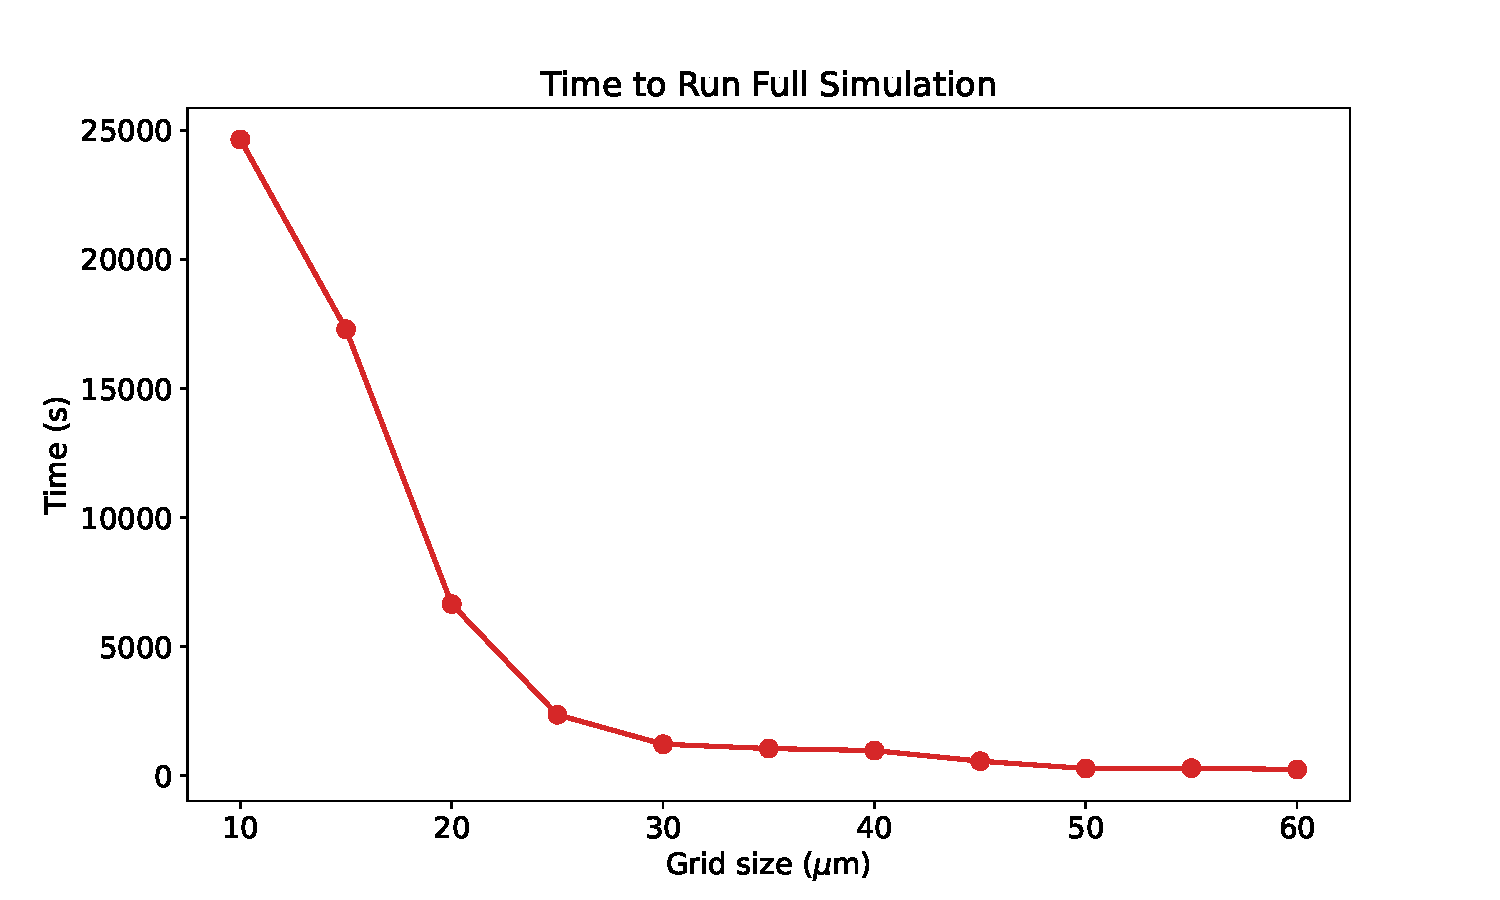
\includegraphics[width=0.99\linewidth]{ch4/figs/cpu_run_time.pdf}
\caption{Run time for a single {\ehd} event on CPU. Run time based on a single compute server in the Longleaf cluster at the University of North Carolina at Chapel Hill.}
\label{fig:CPU_time}
\end{figure}

One way to speed up {\ehd} is by using parallel calculations with Graphic Processing Units (GPUs). We can transform the entire detector into the GPU memory so that each GPU kernel represents a grid point. Then we can perform the calculations at each grid point in parallel, and instead of going through the program one grid point at a time, the points can be updated simultaneously. We executed this strategy using the NVIDIA CUDA {\cpp} framework. Of all the steps executed by {\ehd}, it is expected that performing the relaxation algorithm on the GPU would have the greatest improvement in run time. We thus begin with a discussion of 2-D Poisson equation solvers based on iterative relaxation methods, then explain how we adapted them to GPU architectures.

\section{Iterative Relaxation Algorithms for Solving 2-D Poisson Equation}
\label{ch4_sec_relax_algo}
The electric potential inside the detector can be solved by solving the Poisson equation:

\begin{equation}
    \nabla^2 \phi= -\frac{\rho}{\epsilon},
\end{equation}
\noindent
where $\phi$ is the electrostatic potential, $\epsilon$ is the permittivity of the material, and $\rho$ is the charge density. An analytic solution to the Poisson equation does not exist for most geometries, and we rely on numerical techniques to approximate a solution. To solve for the potential in the {\ehd}, the detector is divided into grid points and assigned the following classification: Point Contact (PC), High Voltage Contact (HVC), Inside the detector, On the Passivated Surface (Passive), Pinchoff points, Ditch, Ditch Edge, and Contact Edge. We treat each point type separately in solving for the potential. The boundary conditions are determined by the geometry of the detector and the impurity concentration. For the passivated surface, the boundary condition is a reflection symmetry about that surface. The impurity concentration on the passivated surface is modified to include the effects of surface charge if present. In the absence of surface charge, this means that the electric field lines at the passivated surface are parallel to the surface. Points on the high-voltage (HV) and point-contact (PC) surfaces have Dirichlet boundary conditions fixed at the contact voltages.

\subsection*{Jacobi method}
A simple way to solve for the potential is to set the boundary condition, run through all the points in the grid, and estimate the solution at a point in the grid by the average of four points around it. The code continues to iterate through the detector, updating all the points until the difference $\phi_{i,j}^{n}$ - $\phi_{i,j}^{n-1}$ at n$^{\text{th}}$ iteration at all points is less than the convergence threshold. This method is called the Jacobi method, and the points are updated using equation \ref{jacobi} \cite{Varga2000}. 

In this method, the iteration order through the points must be fixed: the method begins with the bottom leftmost point. Then it progresses through the row from left to right and repeats, moving up a row each time.


\begin{equation}{\label{jacobi}}
 \phi_{i,j}^{n} = \frac{1}{4}  \left(\phi^{n-1}_{i+1,j} + \phi^{n-1}_{i-1,j} + \phi^{n-1}_{i,j+1} + \phi^{n-1}_{i,j-1} \right)
\end{equation}
Here the $n$ denotes the iteration number, $i$ and $j$ are the radii and height of the grid point under consideration. 

\subsection*{Gauss-Seidel Method}
Although the Jacobi method works well to obtain a numerical solution, it is slow. One way to speed up the method is to use the newly calculated grid points to update the current grid. This is represented by equation \ref{gs_eq} and is termed the Gauss-Seidel method \cite{Varga2000}.

\begin{equation}{\label{gs_eq}}
 \phi_{i,j}^{n} = \frac{1}{4}  \left(\phi^{n-1}_{i+1,j} + \phi^n_{i-1,j} + \phi^{n-1}_{i,j+1} + \phi^n_{i,j-1} \right)
\end{equation}
By incorporating updated values as soon as they are available, Gauss--Seidel converges faster than the Jacobi method.

\subsection*{Successive over-relaxation}
A way to achieve faster convergence with the Gauss-Seidel method is to use a relaxation factor $\omega$ to extrapolate the solution and accelerate the convergence rate. The successive over-relaxation method (SOR) was developed by David Young \cite{Young1950}. It is represented by equation \ref{sor_eq} and helps to reach convergence quickly. It is the method used in {\siggen} simulations to calculate the electric potential. The value of $\omega$ can be between $1$ and $2$, and there is an optimal value that gives the fastest convergence. For most PDE problems, $\omega$ is typically slightly less than 2. Equation \ref{sor_eq} was empirically tuned to approach a value of less than 2 for large detectors while remaining stable for smaller detectors.

\begin{equation}{\label{sor_eq}}
 \phi_{i,j}^{n} = (1-\omega)\phi^{n-1}_{i,j} + \frac{\omega}{4} \left(\phi^{n-1}_{i+1,j} + \phi^n_{i-1,j} + \phi^{n-1}_{i,j+1} + \phi^n_{i,j-1} \right)
\end{equation}


\begin{equation}{\label{omg}}
\omega = \frac{1.991 - 1500.0}{L*R}
\end{equation}

The CPU version of {\ehd} was written using the SOR algorithm, which proved to be quite effective at reaching fast convergence; however, this cannot be parallelized on GPU. This is because when a grid point is updated, a combination of new values ($\phi^{n}$) and old ($\phi^{n-1}$) values is used, as shown in figure \ref{fig:sor_methods}. This cannot be implemented in parallel, as the order of update is significant for the SOR method, and thus cannot be parallelized.


\begin{figure}[!htb]
\centering
 \vspace{0.2cm}
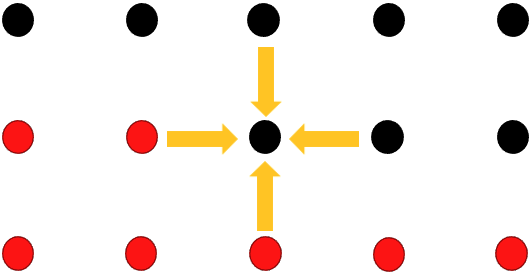
\includegraphics[width=0.4\linewidth]{ch4/figs/SOR.png}
\vspace{0.3cm}
\caption{\label{fig:sor_methods} Updating grid points in the SOR method. Red grid points represent all the points that have already been updated. A given grid point is updated using a mixture of old and new values.}
\end{figure}

\subsection*{Red-Black Successive Over-Relaxation}
To achieve parallelism, we can use a modified SOR algorithm termed Red-Black Successive Over-Relaxation (RB-SOR) \cite{Alefeld1982}. In RB-SOR, we assign a point as red if (i + j) is even and black if (i + j) is odd. We update all the red points using old values and then use the newly updated red values to update the black nodes.

\begin{figure}[!htb]
\centering
 \vspace{0.2cm}
 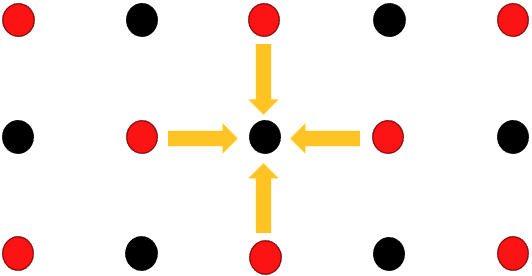
\includegraphics[width=0.4\linewidth]{ch4/figs/RB-SOR.png}
 \vspace{0.3cm}
\caption{\label{fig:rb_sor_methods} Updating grid points in Red-Black SOR. All the red grid points are updated in parallel using old values, and the black grid points are updated using the new red grid points.}
\end{figure}

Figure \ref{fig:rb_sor_methods} shows how RB-SOR differs from traditional SOR. This method reaches convergence in about the same number of iterations as SOR, but the update at each iteration can now be done in parallel using GPUs. Parallel reduction techniques can be used to verify convergence by finding the maximum difference per point between the $\text{n}$ and $\text{n}-1$ iterations. The update equations of the RB-SOR method are:

\begin{equation}{\label{rb_e}}
 \phi_{i,j}^{n} = (1-\omega)\phi^{n-1}_{i,j} + \frac{\omega}{4} \left(\phi^{n-1}_{i+1,j} + \phi^{n-1}_{i-1,j} + \phi^{n-1}_{i,j+1} + \phi^{n-1}_{i,j-1} \right) \qquad \text{ i+j is even}
\end{equation}

\begin{equation}{\label{rb_o}}
 \phi_{i,j}^{n} = (1-\omega)\phi^{n-1}_{i,j} + \frac{\omega}{4} \left(\phi^{n}_{i+1,j} + \phi^n_{i-1,j} + \phi^{n}_{i,j+1} + \phi^n_{i,j-1} \right) \qquad \text{ i+j is odd}
\end{equation}

\begin{figure}[!htb]
\centering
 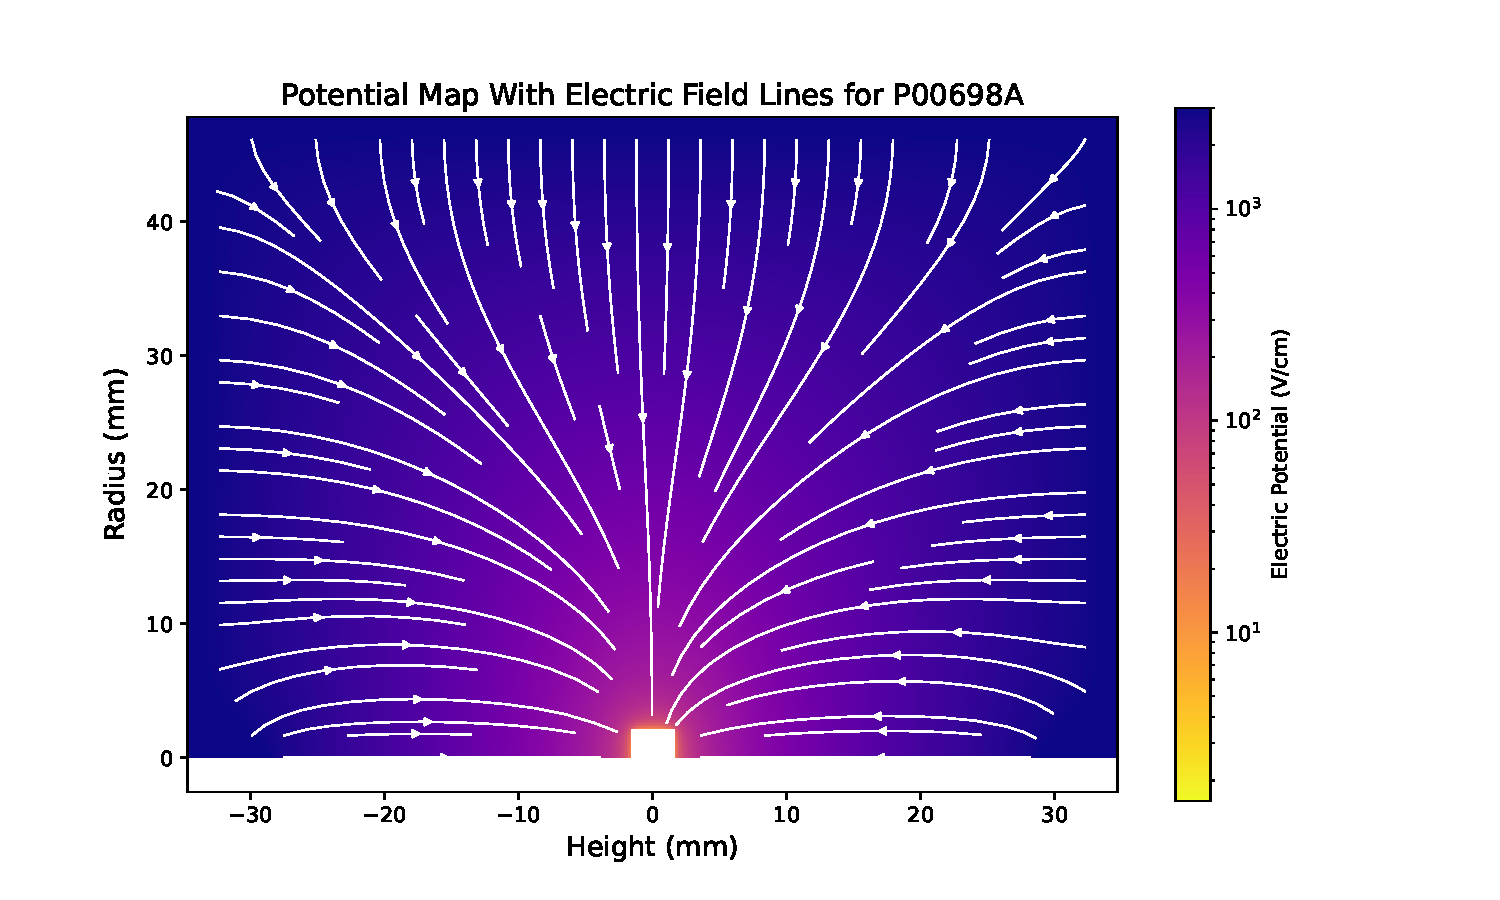
\includegraphics[width=\linewidth]{ch4/figs/elect_pot_P00698A.pdf}
\caption{\label{fig:sor_pot_sol} A solution to the Electric Potential using Red-Black SOR in {\ehd}. The white lines show electric field lines.}
\label{ch4:fig:elect_pot_soln}
\end{figure}

Figure \ref{ch4:fig:elect_pot_soln} shows a solution to the Poisson equation in the program. With the framework set for implementing the relaxation algorithm on the GPU, we are now ready to discuss the programming model used and the parallel computing techniques.


\section{GPU Programming with CUDA {\cpp} }
A Central Processing Unit (CPU) and a Graphics Processing Unit (GPU) are designed with different computations in mind. A CPU is designed to execute a sequence of operations as fast as possible, one at a time, whereas a GPU is designed to execute tens of thousands of operations in parallel. A CPU can perform a single task significantly faster than a GPU, but GPUs dramatically reduce run time in problems where parallelization can be established, such as adding vectors, manipulating matrices, finding gradients, etc. Thus, GPUs are extensively used in areas such as computer vision, gaming, and machine learning. A GPU always needs a CPU to drive the workflow. 

For our purpose, we used NVIDIA GPUs. The Compute Unified Device Architecture (CUDA) is a programming environment that allows writing {\cpp} code on GPUs. CUDA extends the standard {\cpp} environment to enable functions, called kernels, to be executed in parallel by many threads. The GPU performs calculations in the kernel, which contains the sets of instructions each thread has to follow. The kernel execution is divided into blocks, each with a given number of threads, shown in figure \ref{fig:GPU_basics_a}. To enable parallelism, we need to break down the problem onto the GPU grid and then write instructions for threads and blocks to follow.

\begin{figure}
 \begin{subfigure}{0.48\textwidth}
 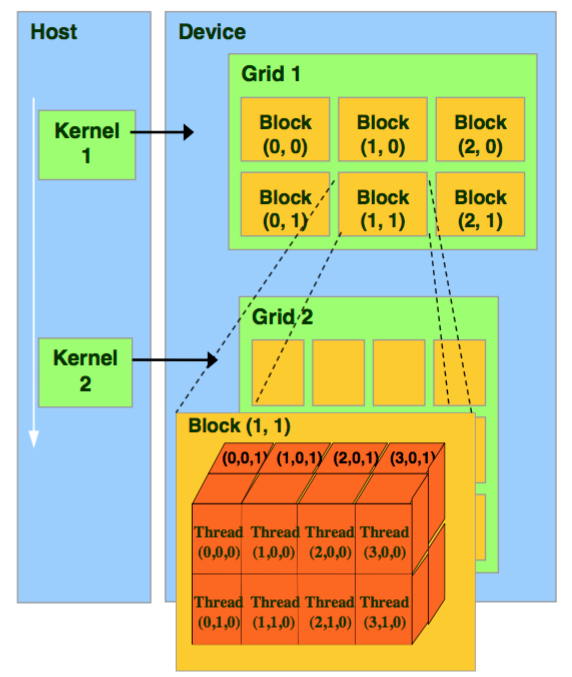
\includegraphics[width=\linewidth]{ch4/figs/grid-of-thread-blocks.png}
 \caption{Computing nodes organized by blocks and threads.} \label{fig:GPU_basics_a}
\end{subfigure}%
\hspace*{\fill}   % maximizeseparation between the subfigures
 \begin{subfigure}{0.48\textwidth}
 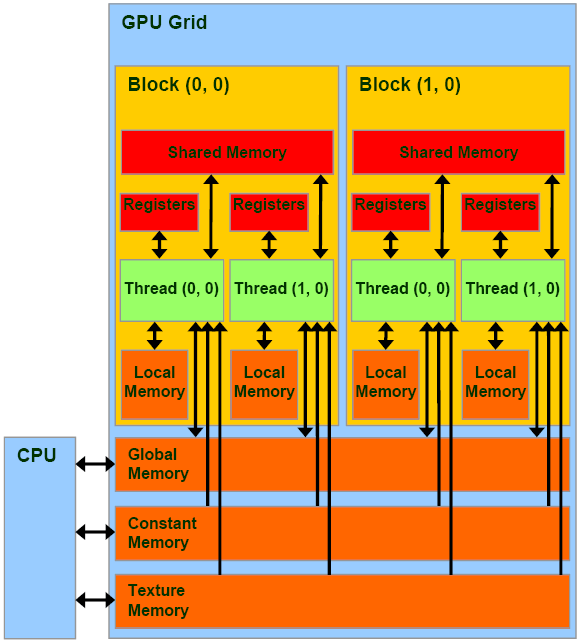
\includegraphics[width=\linewidth]{ch4/figs/memory-hierarchy.png}
 \caption{Memory structure showing global and shared memory.} \label{fig:GPU_basics_b}
 \end{subfigure}
\caption{A depiction of the GPU architecture. Source: NVIDIA CUDA {\cpp}  Programming Guide} \label{fig:GPU_basics}
\end{figure}

In CUDA, the maximum number of blocks that can be called is $65535$ and the maximum number of threads per block is $1024$. We thus want to find a way to split our detector into blocks and threads and index it appropriately for each grid point (r, z). Our first attempt was to set the height z as the block index and the radius r as the grid index such that z$=10$, r$=15$ corresponds to block $10$ and thread $15$. The z and r values used are in grid units, so we never run into decimal point issues with this approach; however, we quickly ran out of threads on smaller grid sizes because there can be at most $1024$ in a given block. To mitigate the problem, we use modular arithmetic to slice the detector of radius R and height L into rectangles of width R and length = max threads, such that the total number of blocks and grids needed is:

\begin{equation}{\label{nu_b}}
 \text{Number of blocks = R}\times \text{ceiling} \left( \frac{\text{L}}{\text{max threads}} \right) \\
\end{equation}

\begin{equation}{\label{nu_g}}
 \text{Number of threads per block = max threads}
\end{equation}
Here $R$ and $L$ are in terms of the number of grid units. Then for a given (block index) and (thread index), the corresponding r and z are:

\begin{equation}{\label{r_eq}}
 \text{r = (blockIdx) mod R} \\
\end{equation}

\begin{equation}{\label{z_eq}}
 \text{z = floor}\left(\frac{\text{blockIdx}}{\text{R}}\right) \times \text{max threads + threadIdx}
\end{equation}

With the blocks and grid framework in place, we can focus on memory management. The GPU memory exists in a different space than the CPU memory. To perform any calculation, we need to copy the data to GPU memory, perform the task with GPUs, and copy the data back to CPU memory. This copying operation is slow, so we aim to minimize the number of copying steps as much as possible. We assigned constants such as grid size, radius, height, etc. to the small shared memory such that both the GPU and CPU can access them simultaneously. Larger arrays such as potentials, point types, and impurities were copied to the large GPU global memory. The GPU also does not perform well on multidimensional arrays, so we flattened them using the formula:

\begin{equation}{\label{flat_array}}
 \text{Array[i][j][k] = flat array[(i} \times \text{(L+1)}\times \text{(R+1))+((R+1)}\times \text{j)+k]}
\end{equation}

The nvcc library was used to compile and link the GPU {\cpp} code with the {\ehd} C code. Using GPUs only for the relaxation algorithm, we achieved a $13$x speed improvement over the CPU-based program. In the new program, the most computationally expensive task was copying between CPU and GPU memory, which was performed every time step after field recalculation. The run time could be reduced by copying all the data needed at the beginning of the program, performing all the necessary calculations on the GPU, and copying back only the required data. This required the implementation of the diffusion and charge drift components and signal calculation on the GPU. Running on the GPU does not result in significantly faster run time for these components, but it does reduce the memory transfer at each step, significantly decreasing the run time.

Performing diffusion and self-repulsion in parallel requires one to address one issue: the interference of threads with each other. When densities are allowed to drift and diffuse, two densities could end up on the same grid point. This would not be an issue on the CPU since points are addressed sequentially, but on the GPU, this would mean that two threads are trying to update the same memory location. This was enough to cause disagreement between CPU and GPU results. CUDA enables the implementation of `atomic operations', which allow a thread to perform a task that is guaranteed to be performed without interference from other threads. Programming the densities to update using atomic operations fixed the discrepancies between the GPU and CPU with no noticeable time loss.

Warp divergence occurs when threads in the GPU attempt to perform different operations. This can lead to divergent results and can also cause performance problems. To avoid this, we modularized the GPU kernels into smaller executions and added device synchronization between each kernel. This made sure that all threads performed the calculation before moving to a new kernel.

Having diffusion and charge drift running on the GPU enabled the entire time step loop in figure \ref{fig:ehd_flowchart} to run on the GPU without copying back to CPU memory. This required careful tracking of the pointers in GPU memory using a C struct to store the locations of all GPU pointers. This struct is initialized in the time step loop by allocating space in GPU memory and copying the required data into it. The calculations are then performed in GPU memory, and only the required data is transferred to CPU memory.

A final improvement in the run time was achieved by generating the signal on the GPU without the need to write the charge cloud densities to the file. In the initial implementation, the signal was calculated by saving snapshots of the densities during the program, and the snapshots were read later to generate the signal. A faster approach is to calculate the signal collected during each time step on the GPU and skip writing the snapshots to the file. Signal calculation entails summing up the charges collected and multiplying them by the weighting potential. 

On the GPU, such operations can be performed using the parallel reduction technique. In this technique, two elements of the array are grouped in pairs. Each pair is computed in parallel with the others, halving the overall array size in one step. This reduction is continued until there is one final number: the sum in our case. We used the NVIDIA Thrust library to perform sums on the GPU using parallel reduction techniques and generate the signal on the GPU. Now, the only memory that is transferred to the CPU is the final simulated waveform.

\section{GPU Performance Comparisons and Benchmarking}
The GPU program accurately reproduced the CPU results with less than 0.69 $\%$ difference in the waveforms. Figure \ref{ch4_fig_waveform_comp} shows a comparison between the waveforms of the two programs.  The difference is primarily due to the different methods of calculating the electric potential: SOR in the CPU versus RB-SOR in the GPU. As shown in figure \ref{ch4_fig_cov_thres_diff}, it reduced to $0.045\%$ when both simulations were allowed to relax to a threshold of numerical convergence at the double precision level. The default convergence threshold was set to $8\times10^{-4}$ by studying the maximum error and run time for different convergence thresholds.

\begin{figure}[!ht]
\centering
 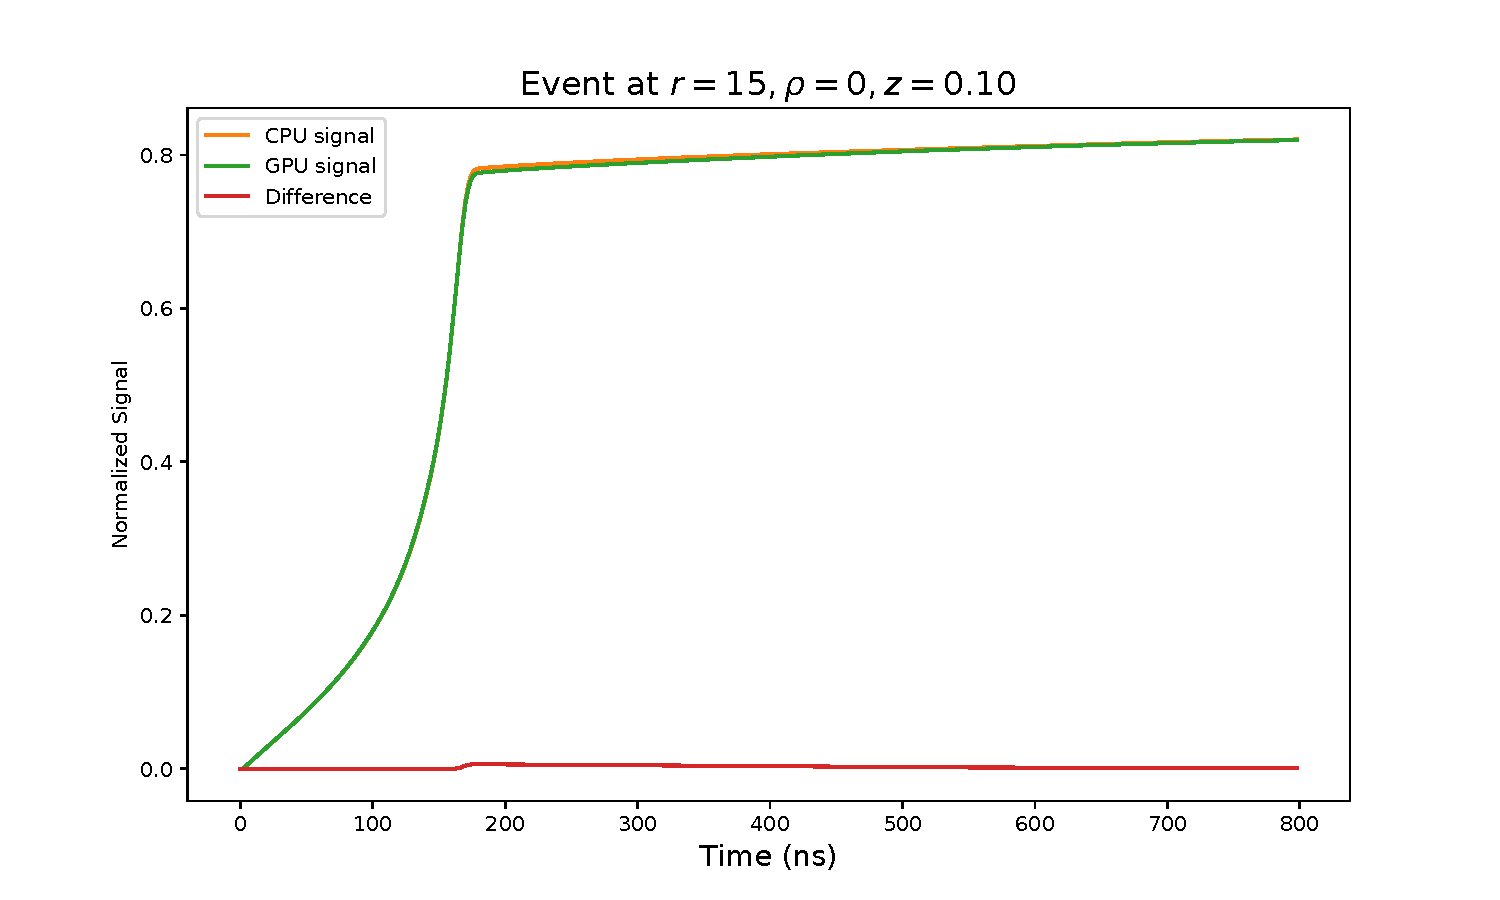
\includegraphics[width=0.99\linewidth]{ch4/figs/cpu_gpu_wf.pdf}
\caption{Comparison of waveform generated by CPU program versus GPU program in {\ehd} at the default converge threshold. The event was at r=$15$mm and z=$0.10$mm.}
\label{ch4_fig_waveform_comp}
\end{figure}

\begin{figure}[!ht]
\centering
 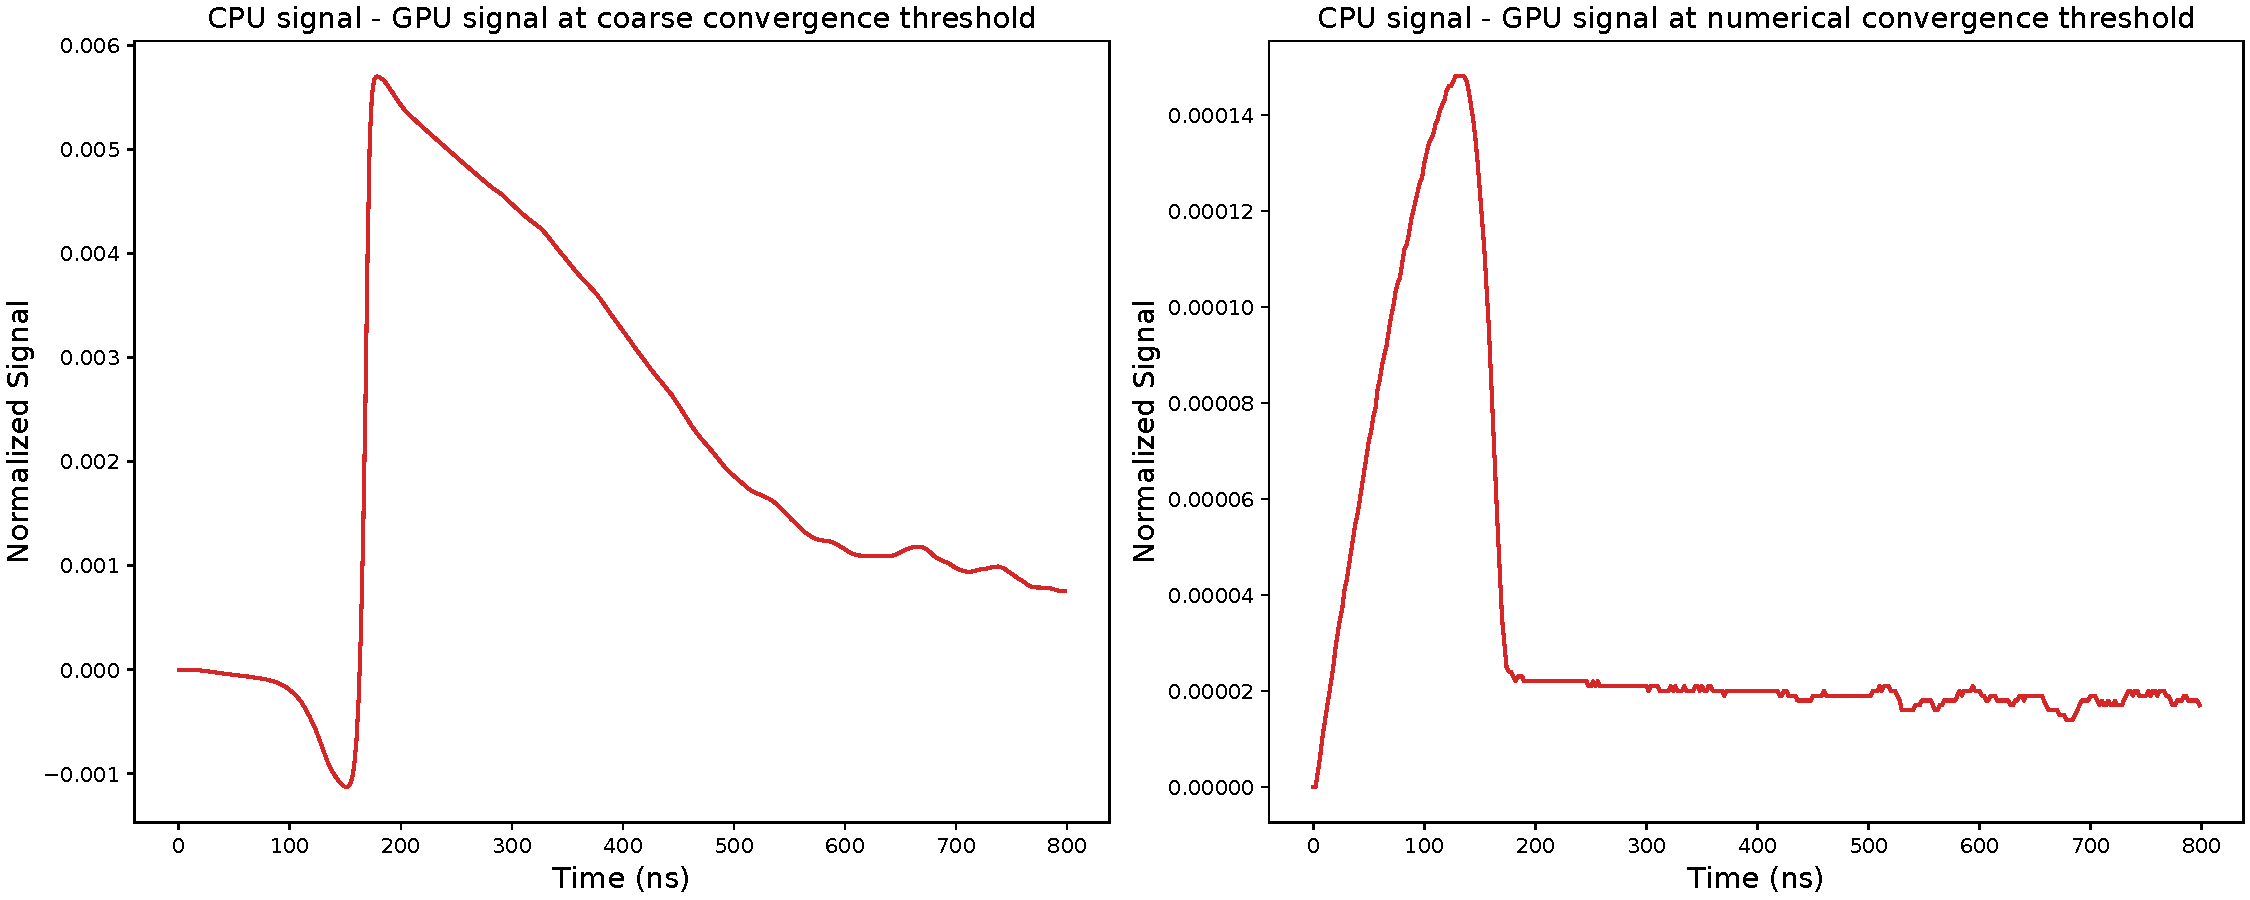
\includegraphics[width=0.99\linewidth]{ch4/figs/converge_threshold_dif.pdf}
\caption{Difference in waveforms produced by the CPU and GPU programs. Left plots shows the difference at default converge threshold for RB-SOR algorithm. Right plot shows the difference at numerical convergence which is set to $8\times10^{-8}$.}
\label{ch4_fig_cov_thres_diff} 
\end{figure}

\begin{figure}[!htb]
\centering
 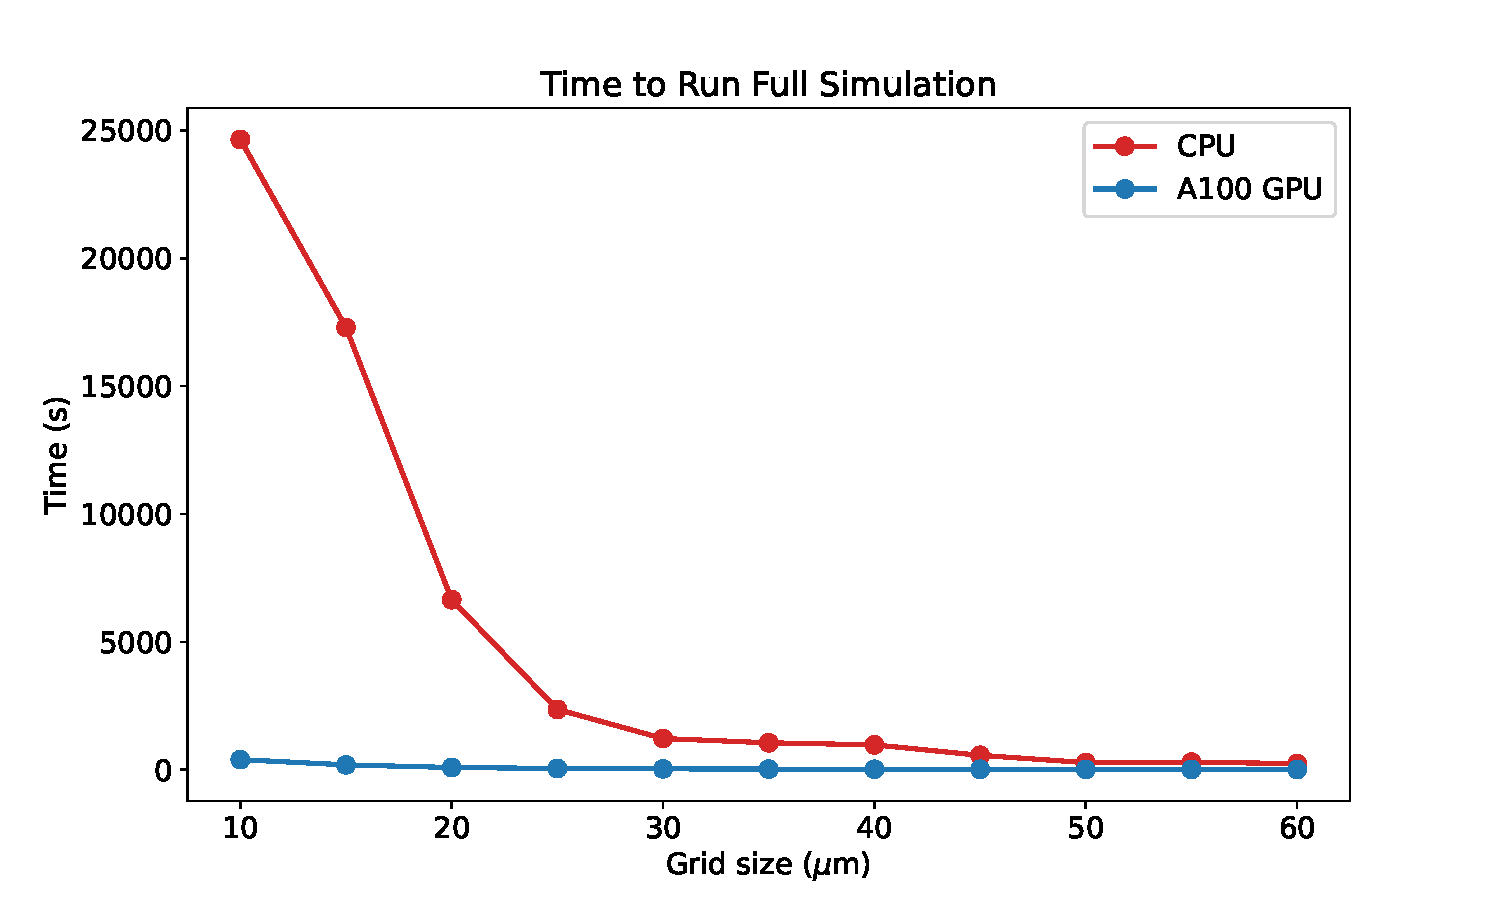
\includegraphics[width=0.99\linewidth]{ch4/figs/cpu_gpu_comp.pdf}
\caption{ Comparison of run time for an {\ehd} event on GPU and CPU. Run times are based on a single CPU node on the Longleaf cluster at UNC-Chapel Hill and an NVIDIA A100 node of the Perlmutter supercomputer at the NERSC.}
\label{fig:GPU_time}
\end{figure}

However, the GPU program was extremely fast, with nearly grid-size-independent execution time. We primarily used GPUs on the Perlmutter supercomputer at the National Energy Research Scientific Computing Center (NERSC). Figure \ref{fig:GPU_time} shows the time taken by each program. For a grid size of $10$ microns, the CPU program took $24642$ seconds ($\sim$ 7 hours) to run, while the GPU program took $394$ seconds ($\sim$ 7 min) to run, representing a speed increase of 62.5x. The biggest contribution to the speed-up was the implementation of the electric potential calculation on the GPU, which was also grid-size independent. Other contributions were the fact that the densities did not have to be written to a file to generate the signal and that there was no need for a transfer of data from GPU memory to CPU memory at each time step. This speed-up will allow for running thousands of simulations and building a waveform library with different configurations.

\begin{figure}[!htb]
    \centering
    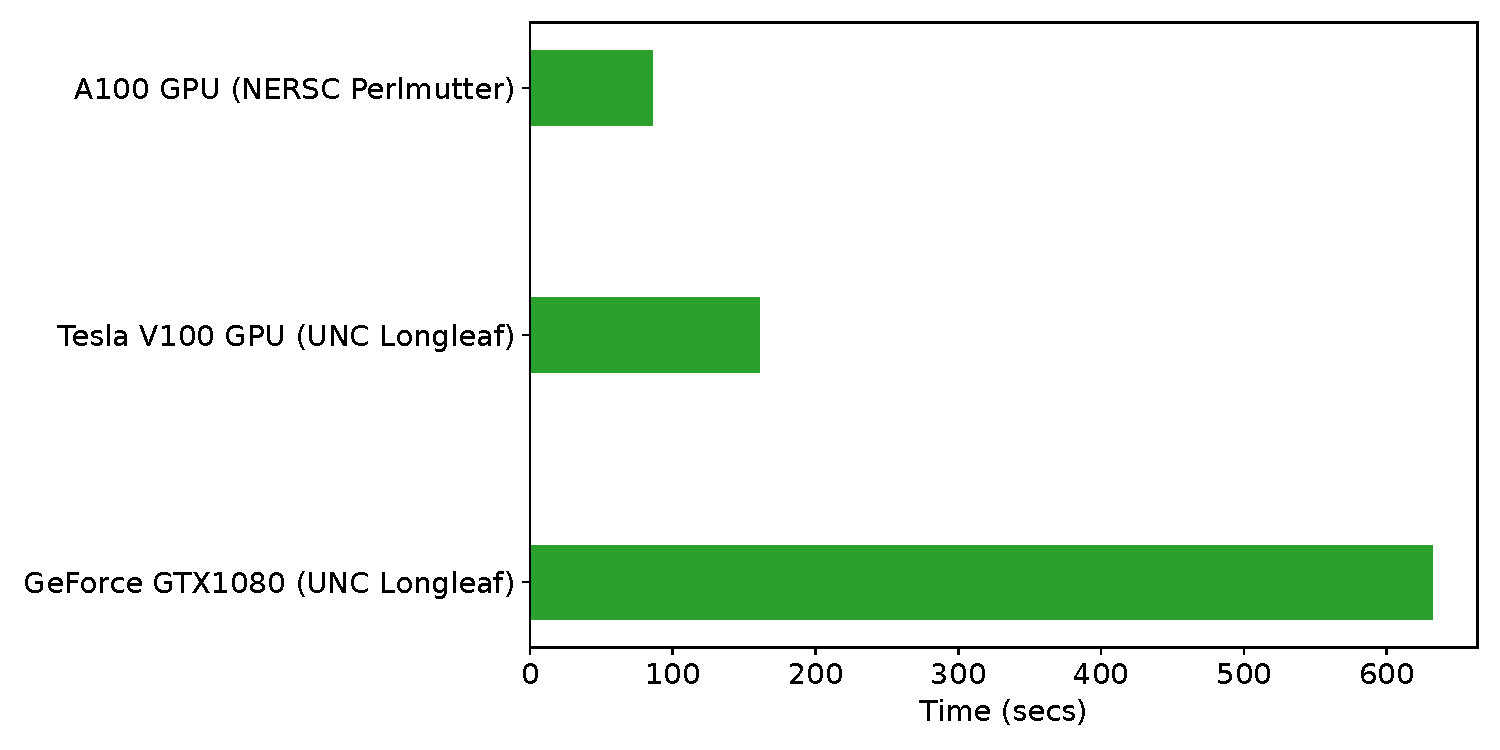
\includegraphics[width=0.99\linewidth]{ch4/figs/gpu_comp.pdf}
\caption{\label{ch4:fig:GPU_comp} Program run time on various GPU models for a $20\mu$ grid. The faster GPU results in lower run time.}
\end{figure}

Figure \ref{ch4:fig:GPU_comp} shows how the run time varies for different NVIDIA GPUs at the two clusters. The faster the GPU, the faster the program runs, suggesting that we have achieved parallelization using sufficient utilization of GPU resources. Table \ref{ch4:tab:gpu_kernels} shows the profiling results of GPU kernels that did not use the standard library. The kernel name is listed alongside its contribution to the total execution time as a percentage time ($\%$), its cumulative execution time in nanoseconds Total Time $(ns)$, and the number of times it was executed during profiling (Instances). The table also includes the average execution time per invocation (Avg $(ns)$), which indicates the computational efficiency of each kernel. Furthermore, the dimensions of the thread blocks (blocks $(x, y, z)$) and the configuration of the grid (grid $(x, y, z)$) are reported. The most computationally intensive kernel was the one in which self-repulsion was performed. This is where we determine where the charges drift to, which can contain many conditional statements and for loops that can slow down GPU performance. This section of the code is an excellent target for further optimization. The kernel that was called the most was the relax step of the RB-SOR algorithm. This is expected as, for a given time step, the program needs to iterate several times to reach convergence. The Block and Grids usage column suggests that we are using x components of the block and grid. This can be improved in the future to use an entire grid, although that would be a computational challenge requiring significant changes to the program. In the next section, we describe some of the results from {\ehd} to show how it can be used to model background events from the passivated surface.

\begin{table}[!ht]
\centering
\renewcommand{\arraystretch}{1.2} % Adjust row height for readability
\setlength{\tabcolsep}{4pt} % Adjust column spacing
\begin{tabular}{|p{0.20\linewidth}|p{0.08\linewidth}|p{0.15\linewidth}|p{0.08\linewidth}|p{0.10\linewidth}|p{0.12\linewidth}|p{0.12\linewidth}|}
\hline
Kernel & Time & Total Time & Insta & Avg & Blocks & Grids \\
 Name &  (\%) & (ns) & -nce &  (ns) & (x,y,z) & (x,y,z) \\
\hline
gpu\_self\_repulsion & 22 & 34341037092& 18594& 1846888 & (1024, 1, 1) & (5211, 1, 1) \\
diff\_update & 16 & 24220569521& 18594& 1302601 & (1024, 1, 1) & (5211, 1, 1) \\
gpu\_sr\_update & 15 & 23512003680& 18594& 1264494 & (1024, 1, 1) & (5211, 1, 1) \\
gpu\_diffusion & 11 & 17148963486& 18594& 922284 & (1024, 1, 1) & (5211, 1, 1) \\
relax\_step & 9 & 14273537269& 51138& 279118& (1024, 1, 1) & (5211, 1, 1) \\
reset\_rho & 5& 7485611884& 18594& 402582 & (1024, 1, 1) & (5211, 1, 1) \\
set\_rho\_zero & 3& 4558563525& 9297& 490326 & (1024, 1, 1) & (5211, 1, 1) \\
update\_impurities & 3& 4455301561& 9297& 479219 & (1024, 1, 1) & (5211, 1, 1) \\
cal\_esum1 & 2& 2996352557& 10898& 274945 & (1024, 1, 1) & (5211, 1, 1) \\
surface\_drift & 1 & 2610854165& 18594& 140413 & (1024, 1, 1) & (5211, 1, 1) \\
cal\_hsum1 & 1 & 2579773466& 10898& 236719 & (1024, 1, 1) & (5211, 1, 1) \\
hvc\_modicication & 1 & 2143933270& 18594& 115302 & (1024, 1, 1) & (5211, 1, 1) \\
cal\_hsum2 & 1 & 1982242036& 10898& 181890 & (1024, 1, 1) & (5211, 1, 1) \\
cal\_esum2 & 1 & 1965082087& 10898& 180315 & (1024, 1, 1) & (5211, 1, 1) \\
surface\_drift\_calc & 1 & 1737101732& 18594& 93422 & (1024, 1, 1) & (5211, 1, 1) \\
z\_relection\_set & 0 & 156035808& 25569& 6102 & (1, 1, 1) & (1736, 1, 1) \\
reflection\_symmetry & 0 & 146862463& 25569& 5743 & (1, 1, 1) & (2543, 1, 1) \\
relax\_step & 0& 62591212& 1332& 46990 & (1024, 1, 1) & (580, 1, 1) \\
set\_passivated\_imp & 0& 11662613& 2295& 5081 & (1, 1, 1) & (1737, 1, 1) \\
z\_relection\_set & 0& 4343140& 666& 6521 & (1, 1, 1) & (579, 1, 1) \\
reflection\_symmetry & 0& 3912788& 666& 5875 & (1, 1, 1) & (848, 1, 1) \\
\hline
\end{tabular}
\caption{Profiling results of custom GPU kernels during simulation. Time values are expressed as percentages and in nanoseconds.}
\label{ch4:tab:gpu_kernels}
\end{table}